\documentclass[10pt,aspectratio=169]{beamer}
\usetheme{default}

\setbeamercovered{invisible}
\setbeamertemplate{navigation symbols}{}
\setbeamertemplate{footline}{
    \flushright{\hfill \insertframenumber{}/\inserttotalframenumber}
}
\usepackage{listings}


\begin{document}
    \title{A discrete (stochastical)\protect\\SIR epidemiological model}
    \author{Alberto Artoni}
    \date{15/03/2023}
    
\begin{frame}[plain, noframenumbering]
    \maketitle
\end{frame}

\begin{frame}{Epidemiological model\footnote{This exercise is inspired by models shown in \\
\url{https://www.washingtonpost.com/graphics/2020/world/corona-simulator/} and \\
\url{https://github.com/seismotologist/coronaVirusContagion}.}}

Consider a discrete population of agents living in a 2D square domain.

\begin{figure}
    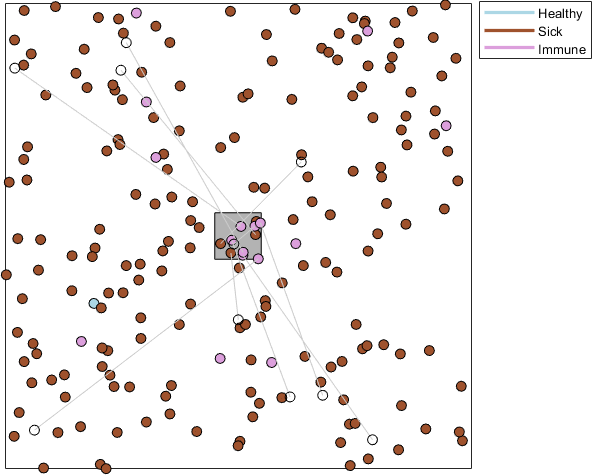
\includegraphics[width=0.5\textwidth]{contagion.png}
\end{figure}
\end{frame}

\begin{frame}{Contagion model}
Starting from random initial positions, the population evolves according to the following rules:

\begin{enumerate}
    \item Each agent can be either \textit{Susceptible}, \textit{Infected} or \textit{Recovered}.
    \item At each timestep, agents move randomly with a given step length.
    \item A prescribed percentage of agents does \textit{social distancing}, i.e. does not move.
    \item Each agent - including those who do social distancing - goes to a pub placed at the center of the domain once every fixed number of time steps.
    \item A \textit{susceptible} agent becomes infected when close to an \textit{infected} agent.
    \item An \textit{infected} agent recovers after a fixed number of time steps.
\end{enumerate}
\end{frame}

\begin{frame}{}
Implementation strategy:
\begin{enumerate}
	\item Create a sketch of the code. 
	\item Get a running version.
	\begin{itemize}
		\item[$\textcolor{blue}{\bullet}$] Each agent will become infected after meeting a susceptible agent.
		\item[$\textcolor{blue}{\bullet}$] There is no pub nor social distancing yet.
		\item[$\textcolor{blue}{\bullet}$] Create a visualization method.
	\end{itemize}
	\item Refine the model.
	\begin{itemize}
		\item[$\textcolor{blue}{\bullet}$] Add the recover dynamics.
		\item[$\textcolor{blue}{\bullet}$] Add the pub and the susceptible.
	\end{itemize}
	\item  Improve the implementation by optimizing the code.
\end{enumerate}
\end{frame}


\begin{frame}{Exercise - Part 0}
	Starting from the given files, implement a \texttt{C++} program that simulates the simplified model. \\
    \begin{itemize}
  		\item[$\textcolor{blue}{\bullet}$] Use an \texttt{enum class} to define the possible agents states.
        \item[$\textcolor{blue}{\bullet}$] Exports the total number of susceptible, infected and recovered agents at each timestep to a \texttt{.csv} file (implement \texttt{Contagion::output\_results}).
        \item[$\textcolor{blue}{\bullet}$] Exports the positions of each agent at each timestep, use a parameter to set the frequency of the export (implement inside \texttt{Contagion::run}).
    \end{itemize}
    
\end{frame}
\begin{frame}{ Exercise - Part 1}  
	Implement now the dynamics of the model.

$\textcolor{blue}{\bullet}$ Each \texttt{Agent} moves at random (implement a \texttt{Agent::move} method). The movement is given by a random direction (implement \texttt{Agent::generate\_random\_step}). If the agent moves outside the domain, the proposed generated step is changed. After $N_{max} = 1000$, if the agent is still going outside the domain, the agent stands still.  \\
\medskip 
$\textcolor{blue}{\bullet}$ The contagion simulation is managed by the method \texttt{Contagion::run} which at each timestep:
        \begin{enumerate}
            \item moves each agent (calls the method \texttt{Agent::move}).
            \item checks the distance between the agents. If one infected agent is close to a susceptible agent, then the susceptible agent becomes infected.
            \item counts the number of agents in each state.
        \end{enumerate}

\end{frame}

\begin{frame}{Exercise - Part 2}
    \begin{itemize}
        \item[\textcolor{blue}{$\bullet$}] Performs the simulation employing the \texttt{<algorithm>} library and parallelize the code using the \texttt{<execution>} library where possible;
        \item[\textcolor{blue}{$\bullet$}] Complete the dynamics of the model by adding the pub and the social distancing. 
    \end{itemize}
    \begin{enumerate}
    	\item Define an enum class for each possible move performed by the agent.
    	\item Add the pub.
    \end{enumerate}
\end{frame}

\begin{frame}{Cache aligment}
    Modern processors use a variety of techniques for performance. Caches is small amount of fast memory where values are ``cached" in hope of reusing recently used or nearby data.
    \begin{figure}
        \centering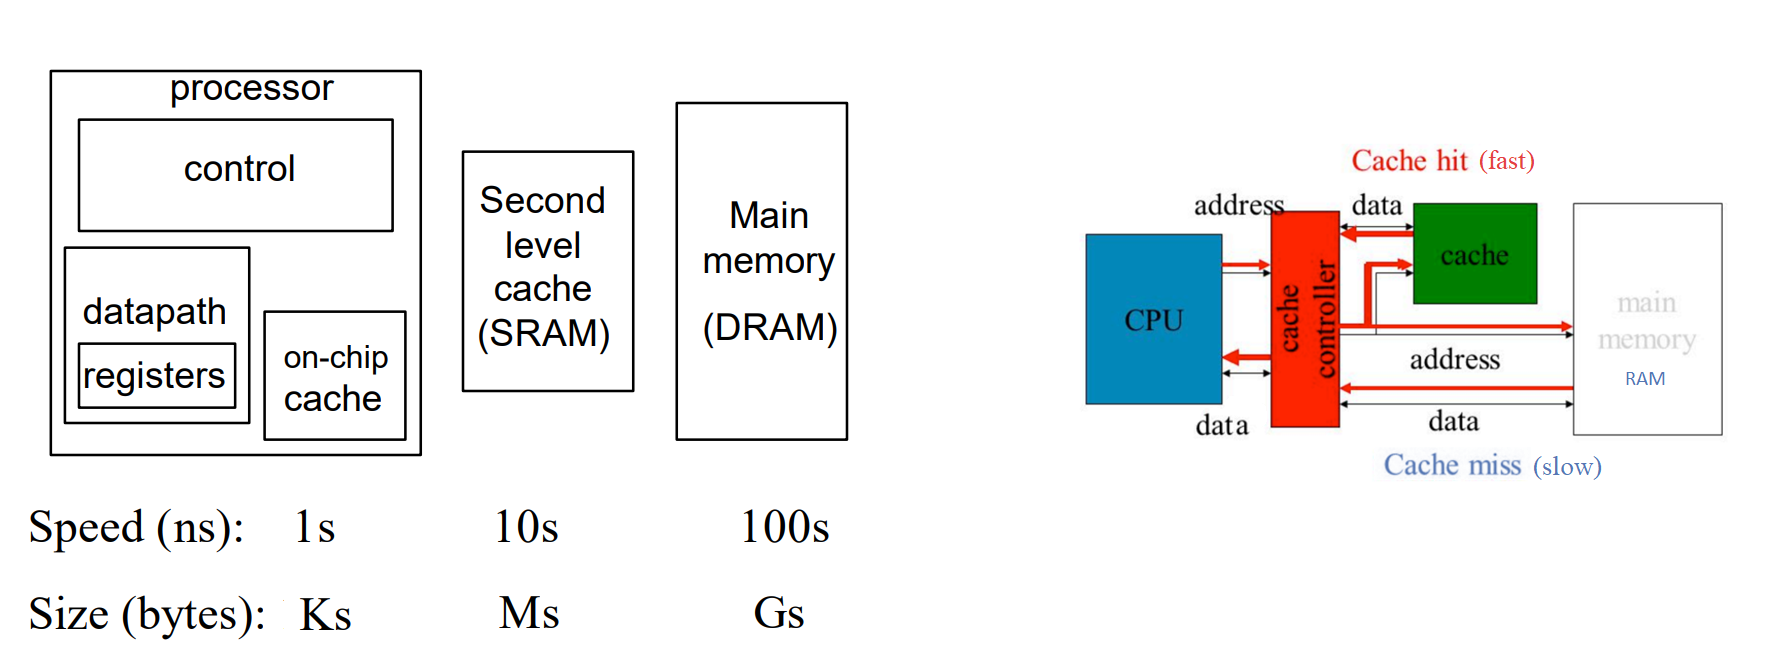
\includegraphics[width=0.8\textwidth]{cache.png}
    \end{figure}
    \begin{itemize}
        \item Taking into account cache aligment is key for linear algebra routines
        \item Libraries like \href{https://github.com/xianyi/OpenBLAS}{OpenBLAS} (which is among the mk modules) or ATLAS are tuned at compile time to take into account hardware specific parameters (like cache size).
        \item \texttt{-O3} aggressive compiler optimization option sometimes is able to do this
    \end{itemize}
\end{frame}

\begin{frame}{Exercise - Part 3}
    Let L1CS be the cache size of a CPU and let $v$ be a large vector of size $K\cdot$L1CS. Consider:
    \lstinputlisting[basicstyle=\footnotesize]{ex1.cpp}
    \begin{itemize}
        \item Optimize the cache alignment for the double for loop used for the radius checking step of the (sequential) simulation.
        \item Use \texttt{getconf -a | grep CACHE} to check the cache size of your PC.
        \item Confront the execution time for different number of agents between the two algorithms.
    \end{itemize}
\end{frame}

\begin{frame}{Possible extensions (homework)}
\begin{enumerate}
    \item Plot the curve of susceptible, infected and recovered using Python, you can read the \texttt{.csv} using the pandas module. You may need to install the matplotlib module with \texttt{pip install matplotlib}.
    \item Create an animation of the positions of the agents at each timestep using Python.
    \item Add social distancing.
    \item Personalize agent-specific parameters, \textit{e.g.}
    \begin{itemize}
        \item by random generation, or
        \item by reading multiple pairs of \{agent index, parameter value\}\\
              for each parameter from file;
    \end{itemize}
    \item Take birth and mortality rates into account.
    \item Extend the model to 3D domains (possibly using templates).
\end{enumerate}
\end{frame}
\end{document}
